\documentclass{standalone}

\usepackage{tikz}
\usepackage{circuitikz}

\tikzset{block/.style = {draw, fill=white, very thick, rectangle, minimum height=1cm, minimum width=2cm},
         lblock/.style={draw,fill=white,very thick, rectangle, minimum height=3cm, minimum width=1cm},
         sum/.style= {draw, fill=white, very thick, circle, node distance=0.5cm}}

         
\begin{document}
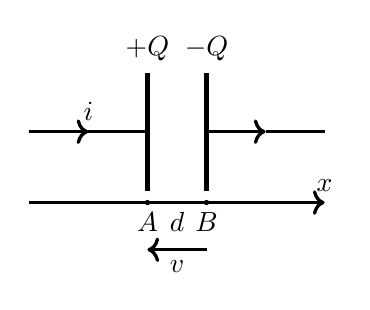
\begin{tikzpicture}[scale=1.5]
    \draw[->,very thick](-1.5,0)--(-1,0)node[above]{$i$};
    \draw[-,very thick](-1,0)--(-0.5,0);
    \draw[-,ultra thick](-0.5,-0.5)--(-0.5,0.5)node[above]{$+Q$};
    \draw[-,ultra thick](0,-0.5)--(0,0.5)node[above]{$-Q$};
    \draw[->,very thick](0,0)--(0.5,0);
    \draw[-,very thick](0.5,0)--(1,0);

    \draw[->,very thick](-1.5,-0.6)--(1,-0.6)node[above]{$x$};
    \filldraw[black](-0.5,-0.6)circle(0.5pt);
    \filldraw[black](0,-0.6)circle(0.5pt);
    \node[below]at(-0.5,-0.6){$A$};
    \node[below]at(0,-0.6){$B$};
    \node[below]at(-0.25,-0.6){$d$};
    \draw[->,very thick](0,-1)--(-0.5,-1)node[midway, below]{$v$};
\end{tikzpicture}
\end{document}